\documentclass[10pt,xcolor=pdflatex,hyperref={unicode}]{beamer}
\usepackage{newcent}
\usepackage[utf8]{inputenc}
%\usepackage[czech]{babel}
%\usepackage[T1]{fontenc}
\usepackage{hyperref}
\usepackage{fancyvrb}
\usetheme{FIT}

\usepackage{setspace}
\usepackage{enumerate}
\usepackage[export]{adjustbox}
\usepackage{wrapfig}
%%%%%%%%%%%%%%%%%%%%%%%%%%%%%%%%%%%%%%%%%%%%%%%%%%%%%%%%%%%%%%%%%%
\title{Efektivní evoluční návrh \\celulárního automatu}

\author[]{
Tomáš Beránek\\
}

%\institute[]{Brno University of Technology, Faculty of Information Technology\\
%Bo\v{z}et\v{e}chova 1/2. 612 66 Brno - Kr\'alovo Pole\\
%login@fit.vutbr.cz}

\institute[]{xberan46@stud.fit.vutbr.cz\\
Fakulta informačních technologií Vysokého učení technického v Brně\\
%Bo\v{z}et\v{e}chova 1/2. 612 66 Brno - Kr\'alovo Pole\\
}

% České logo - Czech logo
% beamerouterthemeFIT.sty řádek 9: fitlogo1_cz

\date{13. května 2022}
%\date{\today}
%\date{} % bez data / without date

%%%%%%%%%%%%%%%%%%%%%%%%%%%%%%%%%%%%%%%%%%%%%%%%%%%%%%%%%%%%%%%%%%


\begin{document}


\frame[plain]{\titlepage}

\begin{frame}
\frametitle{Zadání}
Cílem tohoto projektu je návrh a implementace \emph{efektivního} evolučního algoritmu pro hledání \emph{počáteční konfigurace} 2D celulárního automatu. Celulární automat se řídí pravidly \emph{Game of Life}. Hledaná počáteční konfigurace musí vést v 1 až N krocích do požadované, předem dané, konfigurace.
\end{frame}

\begin{frame}
\frametitle{Implementace}
\doublespacing
\begin{itemize}
    \item inspirace pro EA -- 3. BIN cvičení
    \item hlavní cíle
        \begin{itemize}
            \item optimalizace kódu
            \item návrh nových genetických operátorů
            \item ladění hyperparametrů
        \end{itemize}
\end{itemize}
\end{frame}

\begin{frame}
\frametitle{Optimalizace kódu}
    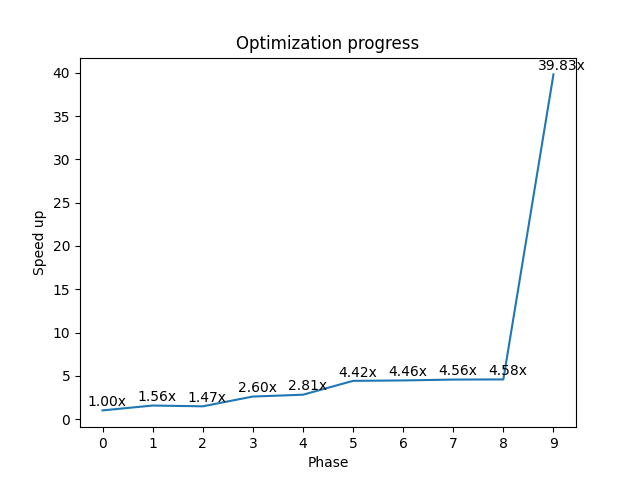
\includegraphics[width=0.8\paperwidth]{img/optimization_progress.png}
\end{frame}

\begin{frame}
\frametitle{Prostorové křížení}
\doublespacing
\begin{itemize}
    \item bodové krížení -- vektory
\end{itemize}
\hspace{0.2cm}
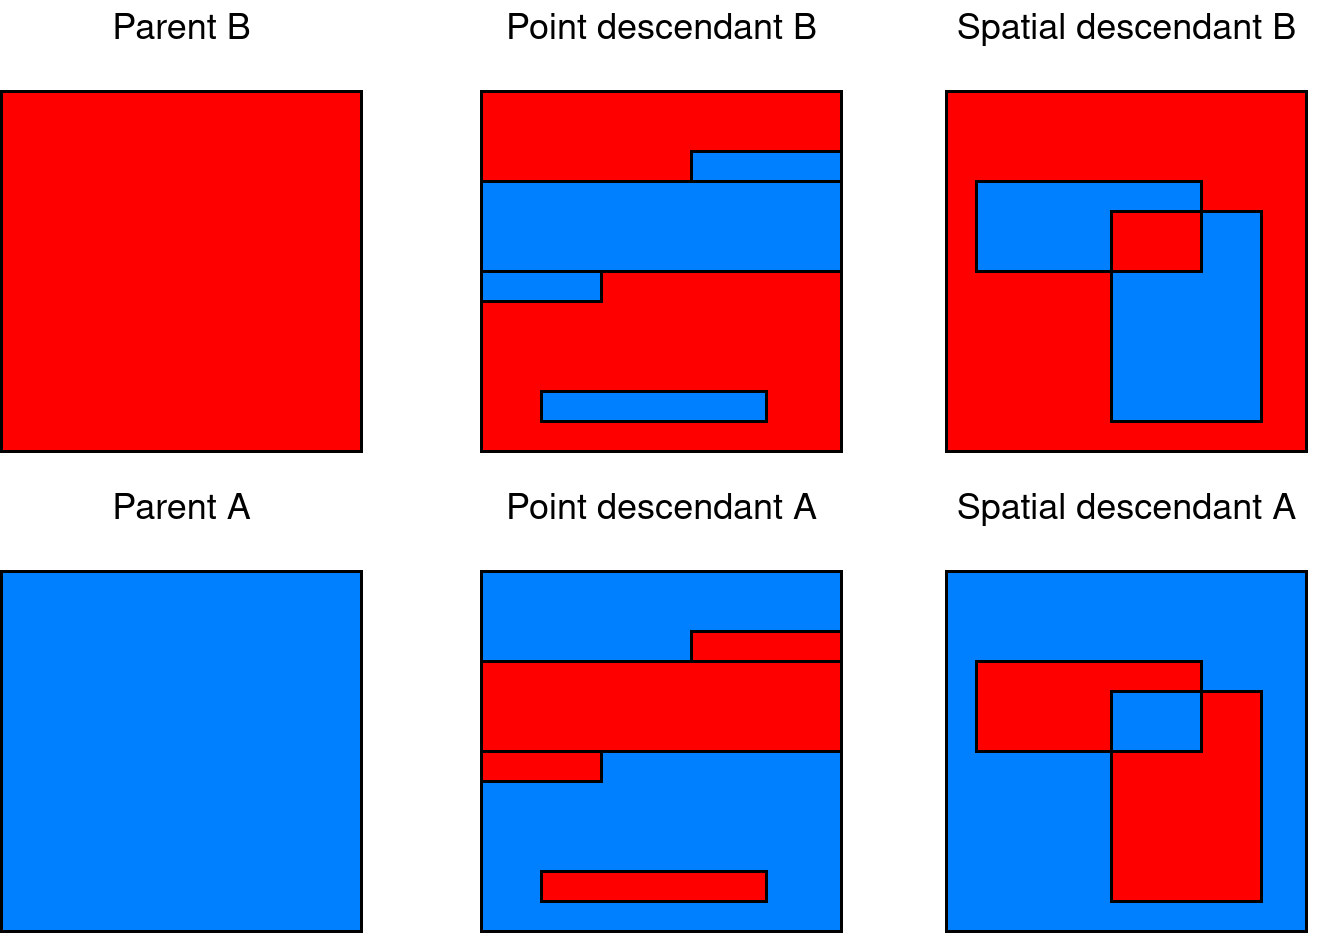
\includegraphics[width=0.8\paperwidth]{img/cross.png}
\end{frame}

\begin{frame}
\frametitle{Prostorová mutace}
\doublespacing
\begin{itemize}
    \item problém vymírání populace
    \item bodová mutace -- příliš řídká na oživení
\end{itemize}
\vspace{1cm}
\hspace{0.2cm}
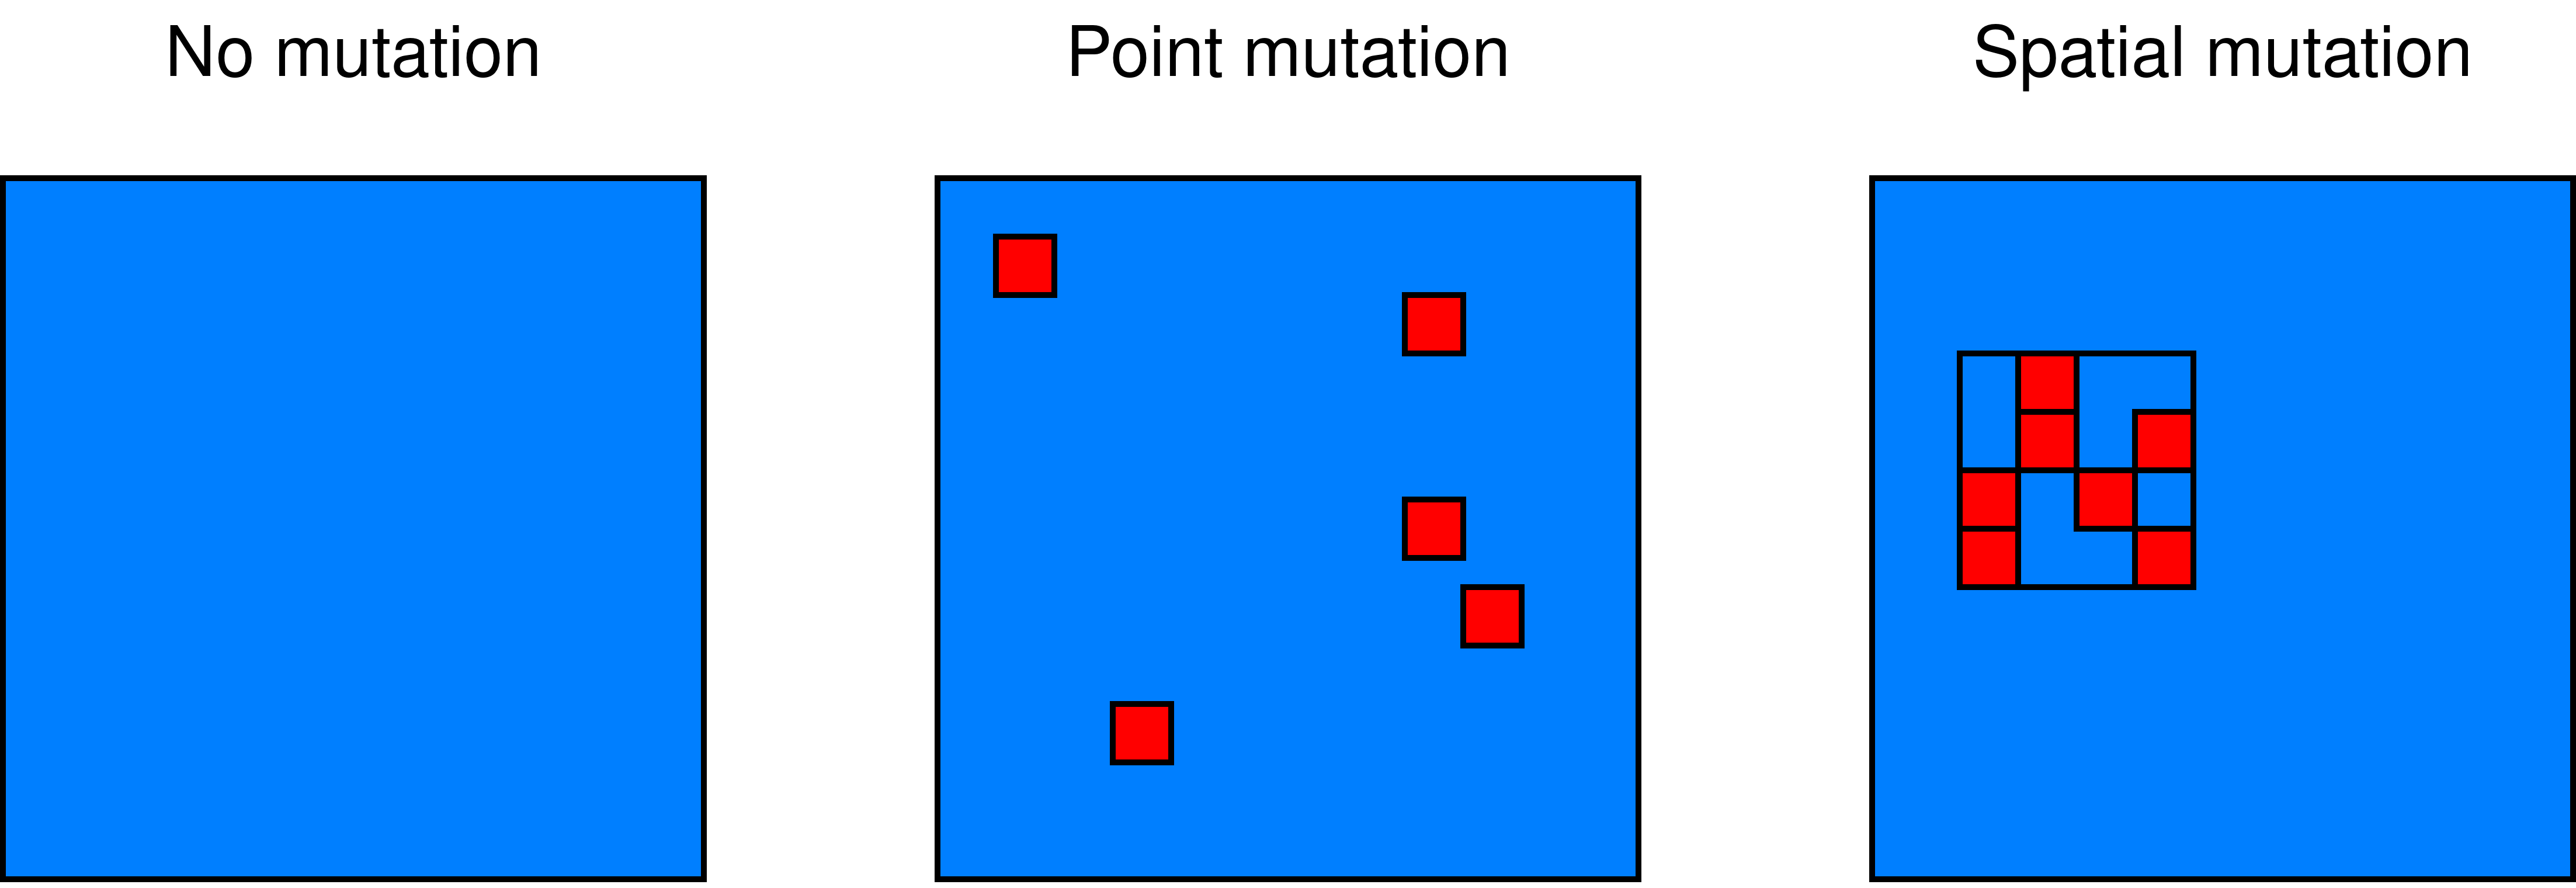
\includegraphics[width=0.8\paperwidth]{img/mutation.png}
\end{frame}

\begin{frame}
\frametitle{Experimenty s bodovými operacemi}
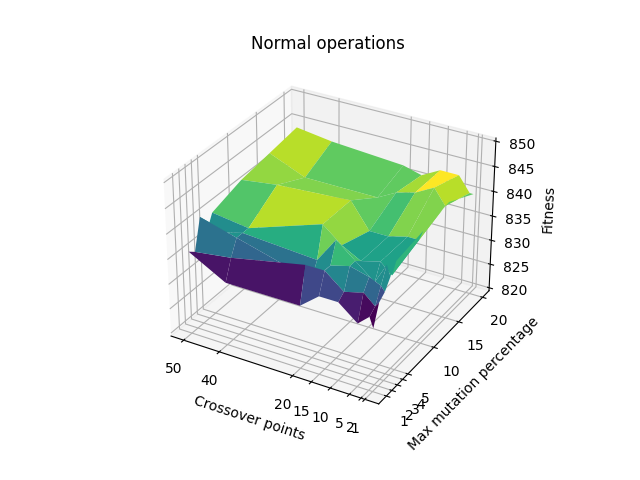
\includegraphics[width=0.8\paperwidth]{img/normal.png}
\end{frame}

\begin{frame}
\begin{itemize}
    \item \emph{nejlepší nastavení} (825) -- 2 obdélníky a 1 mutovaná oblast
\end{itemize}
\frametitle{Experimenty s prostorovými operacemi}
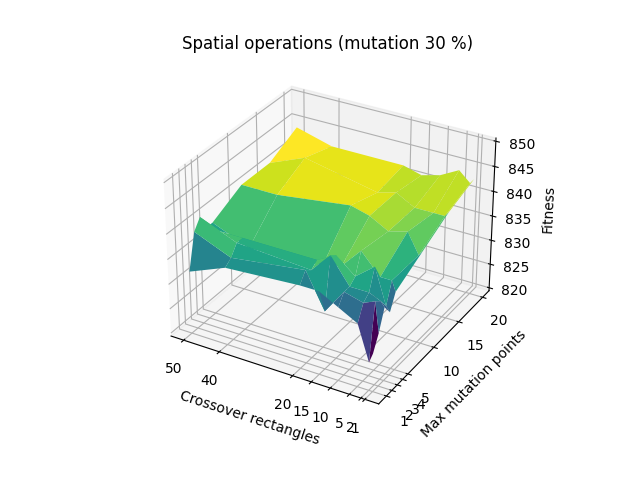
\includegraphics[width=0.8\paperwidth]{img/spatial30.png}
\end{frame}

\begin{frame}
\frametitle{Experimenty s prostorovými operacemi}
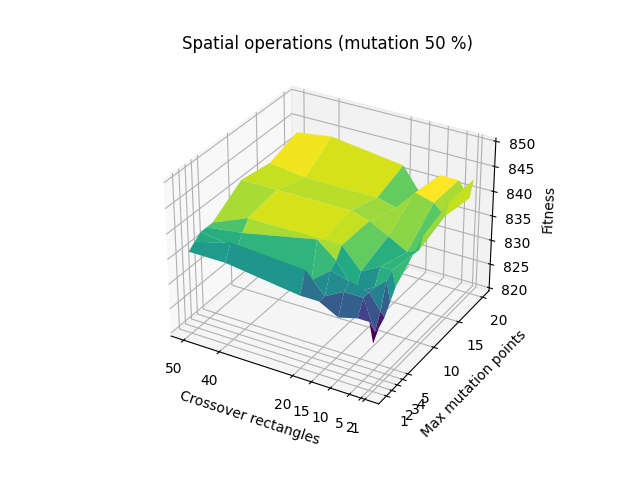
\includegraphics[width=0.8\paperwidth]{img/spatial50.png}
\end{frame}

\begin{frame}
\frametitle{Experimenty s prostorovými operacemi}
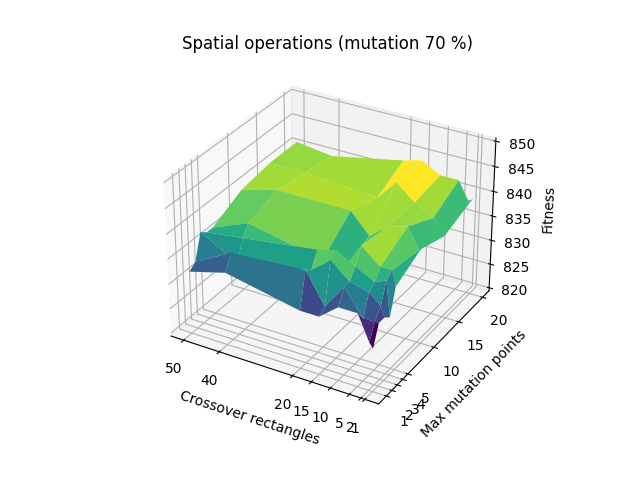
\includegraphics[width=0.8\paperwidth]{img/spatial70.png}
\end{frame}

\begin{frame}
\frametitle{Hledání vhodné velikosti populace}
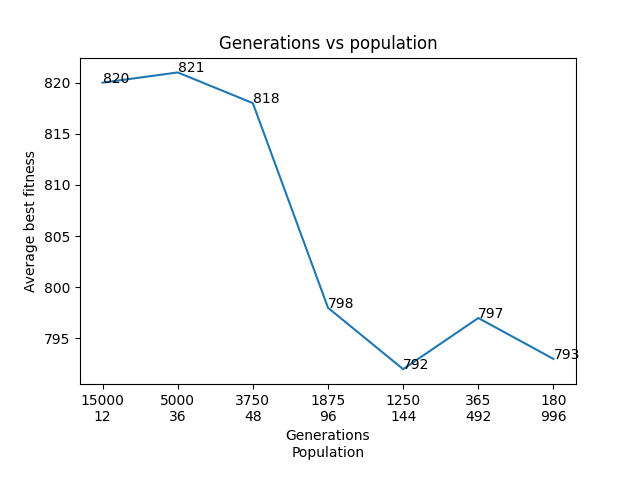
\includegraphics[width=0.8\paperwidth]{img/generations.png}
\end{frame}

\begin{frame}
\frametitle{Závěr}
\doublespacing
\begin{itemize}
    \item cílem byl \emph{efektivní} návrh EA
        \begin{itemize}
            \item kód zrychlen \alert{40x}
            \item rychlejší konvergence u \alert{prostorových operací}
            \item rychlejší konvergence pro \alert{větší populace}
        \end{itemize}
\end{itemize}
\end{frame}


\bluepage{Děkuji Vám za pozornost}

\end{document}
